% Chapter 5

\chapter{Produzione} % Main chapter title

\label{Chapter5} % Change X to a consecutive number; for referencing this chapter elsewhere, use \ref{ChapterX}

%----------------------------------------------------------------------------------------
%	SECTION 1
%----------------------------------------------------------------------------------------

\section{Modellazione}
\begin{itemize}
    \item modelli "lowpoly"
\end{itemize}
\section{Texturing}
\section{Animazione e Rigging}

\begin{figure}
\centering
\begin{subfigure}{.33\textwidth}
  \centering
  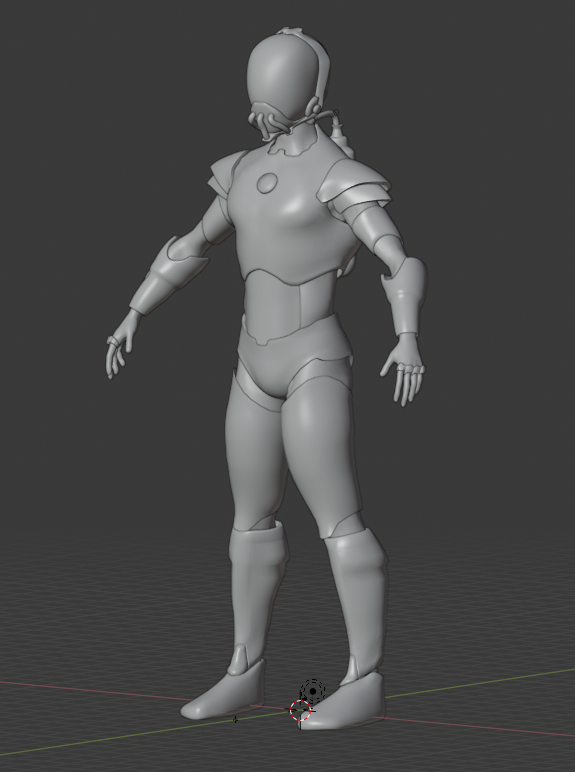
\includegraphics[width=\linewidth]{Figures/rig0}
  \caption{no rig}
  \label{fig:FK1}
\end{subfigure}%
\begin{subfigure}{.33\textwidth}
  \centering
  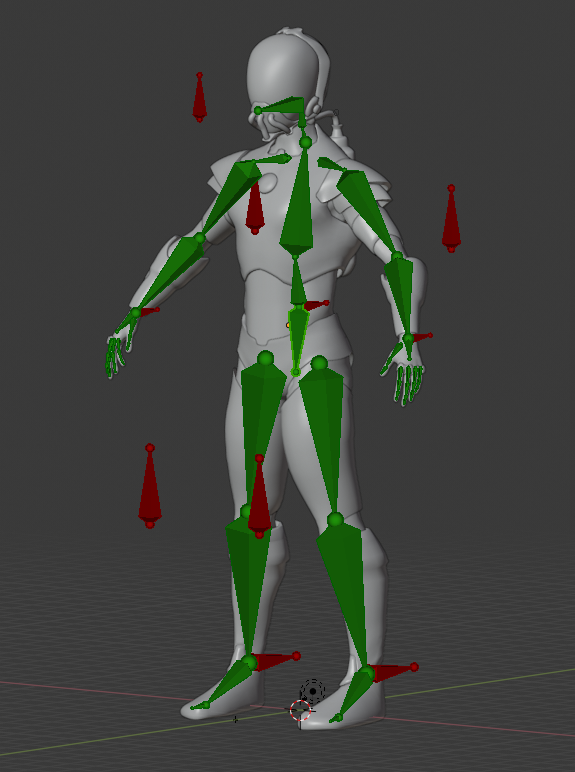
\includegraphics[width=\linewidth]{Figures/rig1}
  \caption{armature}
  \label{fig:FK2}
\end{subfigure}%
\begin{subfigure}{.33\textwidth}
  \centering
  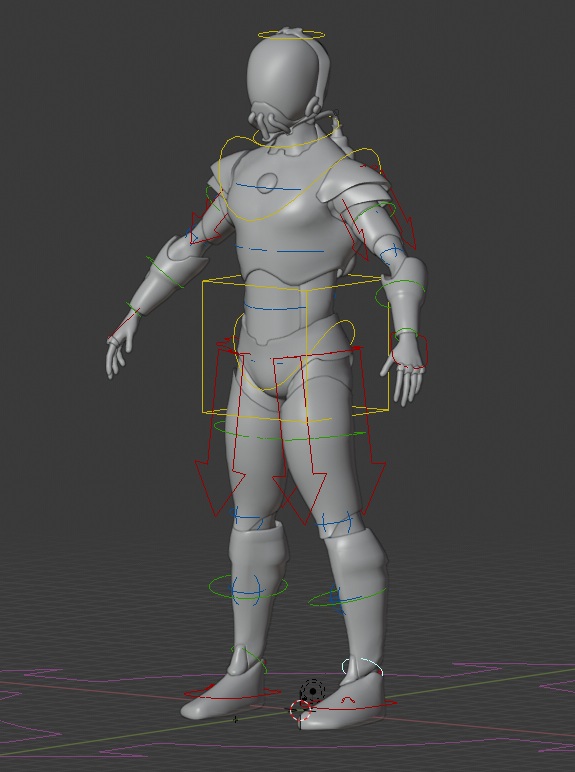
\includegraphics[width=\linewidth]{Figures/rig2}
  \caption{rig}
  \label{fig:FK3}
\end{subfigure}
\decoRule
\caption[Rig]{Esempio di posizionamento tramite Forward Kinematic. La figura rappresenta la stessa armatura, formata da diverse ossa, in tre posizioni differenti.}
\label{fig:FK}
\end{figure}

Rigging è un termine generale che si riferisce all'aggiunta di controlli ad un oggetto, tipicamente allo scopo di animarlo \parencite{blendDoc}.
Consiste nell'assegnare relazioni tra oggetti \parencite{BlendTut}.
\section{Animazione di un corpo umano}
\subsection{Arti superiori}
dita: FK
braccia: mixing FK and IK
         arm should not follow body rotation, but keep the world's space rotation
\subsection{Arti inferiori}
gambe: IK
\section{Espressioni facciali}
uso di shape keys
ogni vertice è importante, inutile associare un'osso per ogni gruppo di vertici: meglio avere diverse espressioni (set finito) e sciegliere quale si vuole usare in ase ad un valore reale (continuo)

dialoghi
menzionare Rhubarb

divisione dx/sx

Reference
\begin{itemize}
    \item Dialog - The Animator's Survival Kit (p.304) 
    \item Facial animation - Algorithms\&Techniques (p.491)
\end{itemize}
\section{Lighting}
\section{Rendering}

